\section{Memoria cache}
In un architettura gerarchica su due livelli, come quella mostrata in figura [\ref{fig:2livmem}], la memoria M1 deve necessariamente essere veloce ed è quindi di tipo statico, mentre la memoria M2, di dimensioni maggiori e destinata tipicamente a contenere tutti i dati e tutte le istruzioni, è di tipo dinamico. Senza scendere troppo in dettagli tecnici, le memorie statiche sono generalmente caratterizzate da un elevato numero di transistor e dimensioni molto ridotte, mentre le memorie dinamiche sono basate su effetti capacitivi e tendono a perdere la carica, dunque devono ricevere processi di refresh che consistono nel riscrivere nuovamente il dato. La prima tipologia di memoria prende convenzionalmente il nome di \textbf{memoria cache}.
\begin{figure}[!h]
    \centering
    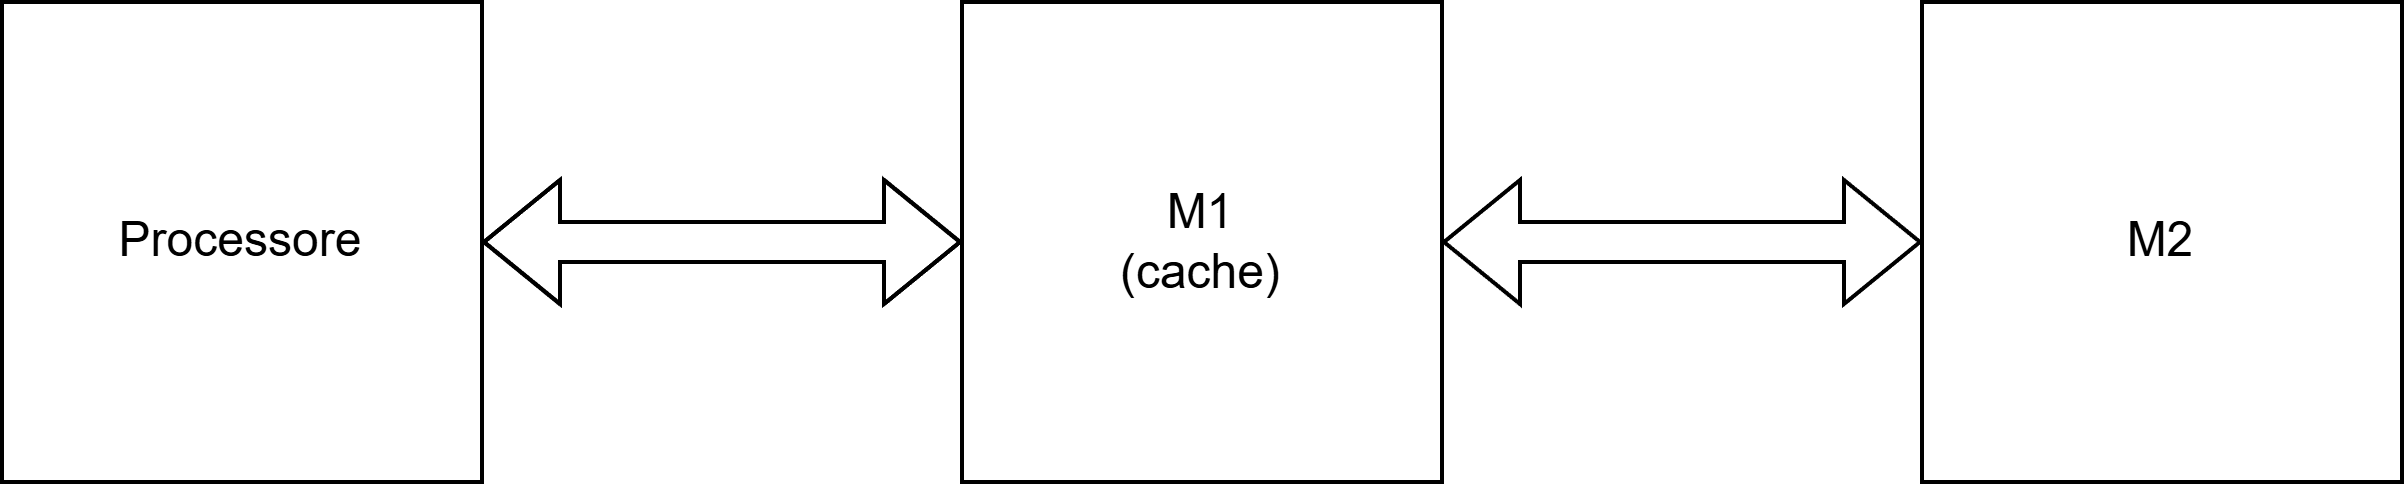
\includegraphics[width=0.6\linewidth]{img/2liv_mem.png}
    \caption{Gerarchia delle memorie su due livelli.}
    \label{fig:2livmem}
\end{figure}

Come ben sappiamo, la memoria centrale lavora con il concetto di indirizzo: viene fornito un valore al decoder e questo fa accedere a una corrispondente locazione di memoria. Questo principio di funzionamento vuole implicitamente afferire che ogni indirizzo è valido, ossia esiste sempre qualche informazione (anche se nulla) contenuta in quest'ultimo. Tale comportamento differisce da quello delle memorie associative, nelle quali una volta fornita la chiave, l'oggetto associato potrebbe non esistere. Le memorie cache funzionano proprio con questa filosofia, sono infatti organizzate in blocchi di dati contigui indicizzati da un'opportuna chiave, detta anche tag. Il motivo della contiguità dei dati nei blocchi va ricercato nel \textbf{Principio di Località} (spaziale), il quale stabilisce che se si accede a un indirizzo di memoria, è probabile che presto saranno necessari dati contenuti in indirizzi vicini. Quando il processore fornisce l'indirizzo dell'informazione a cui accedere questo viene scomposto in due parti: la prima identifica la chiave, mentre la seconda specifica la posizione del dato da prelevare all'interno nel blocco. Se la porzione di chiave individuata non combacia con nessuna delle chiavi presenti, e quindi il corrispondente blocco non è in cache, si verifica un cache miss. Questa prima tipologia di architettura per le memorie cache presentate prende il nome di \textbf{Full Associative} [\ref{fig:full-ass}], ed è una soluzione leggermente più semplice di quella \textbf{Set Associative} presentata di seguito. \MakeUppercase{è} molto importante notare che il processore per accedere a una parola in memoria ne fornisce sempre l'indirizzo, indipendentemente dal fatto che questa si trovi in cache oppure no, in quanto il processore è del tutto trasparente rispetto all'organizzazione delle memoria.

\begin{figure}[!h]
    \centering
    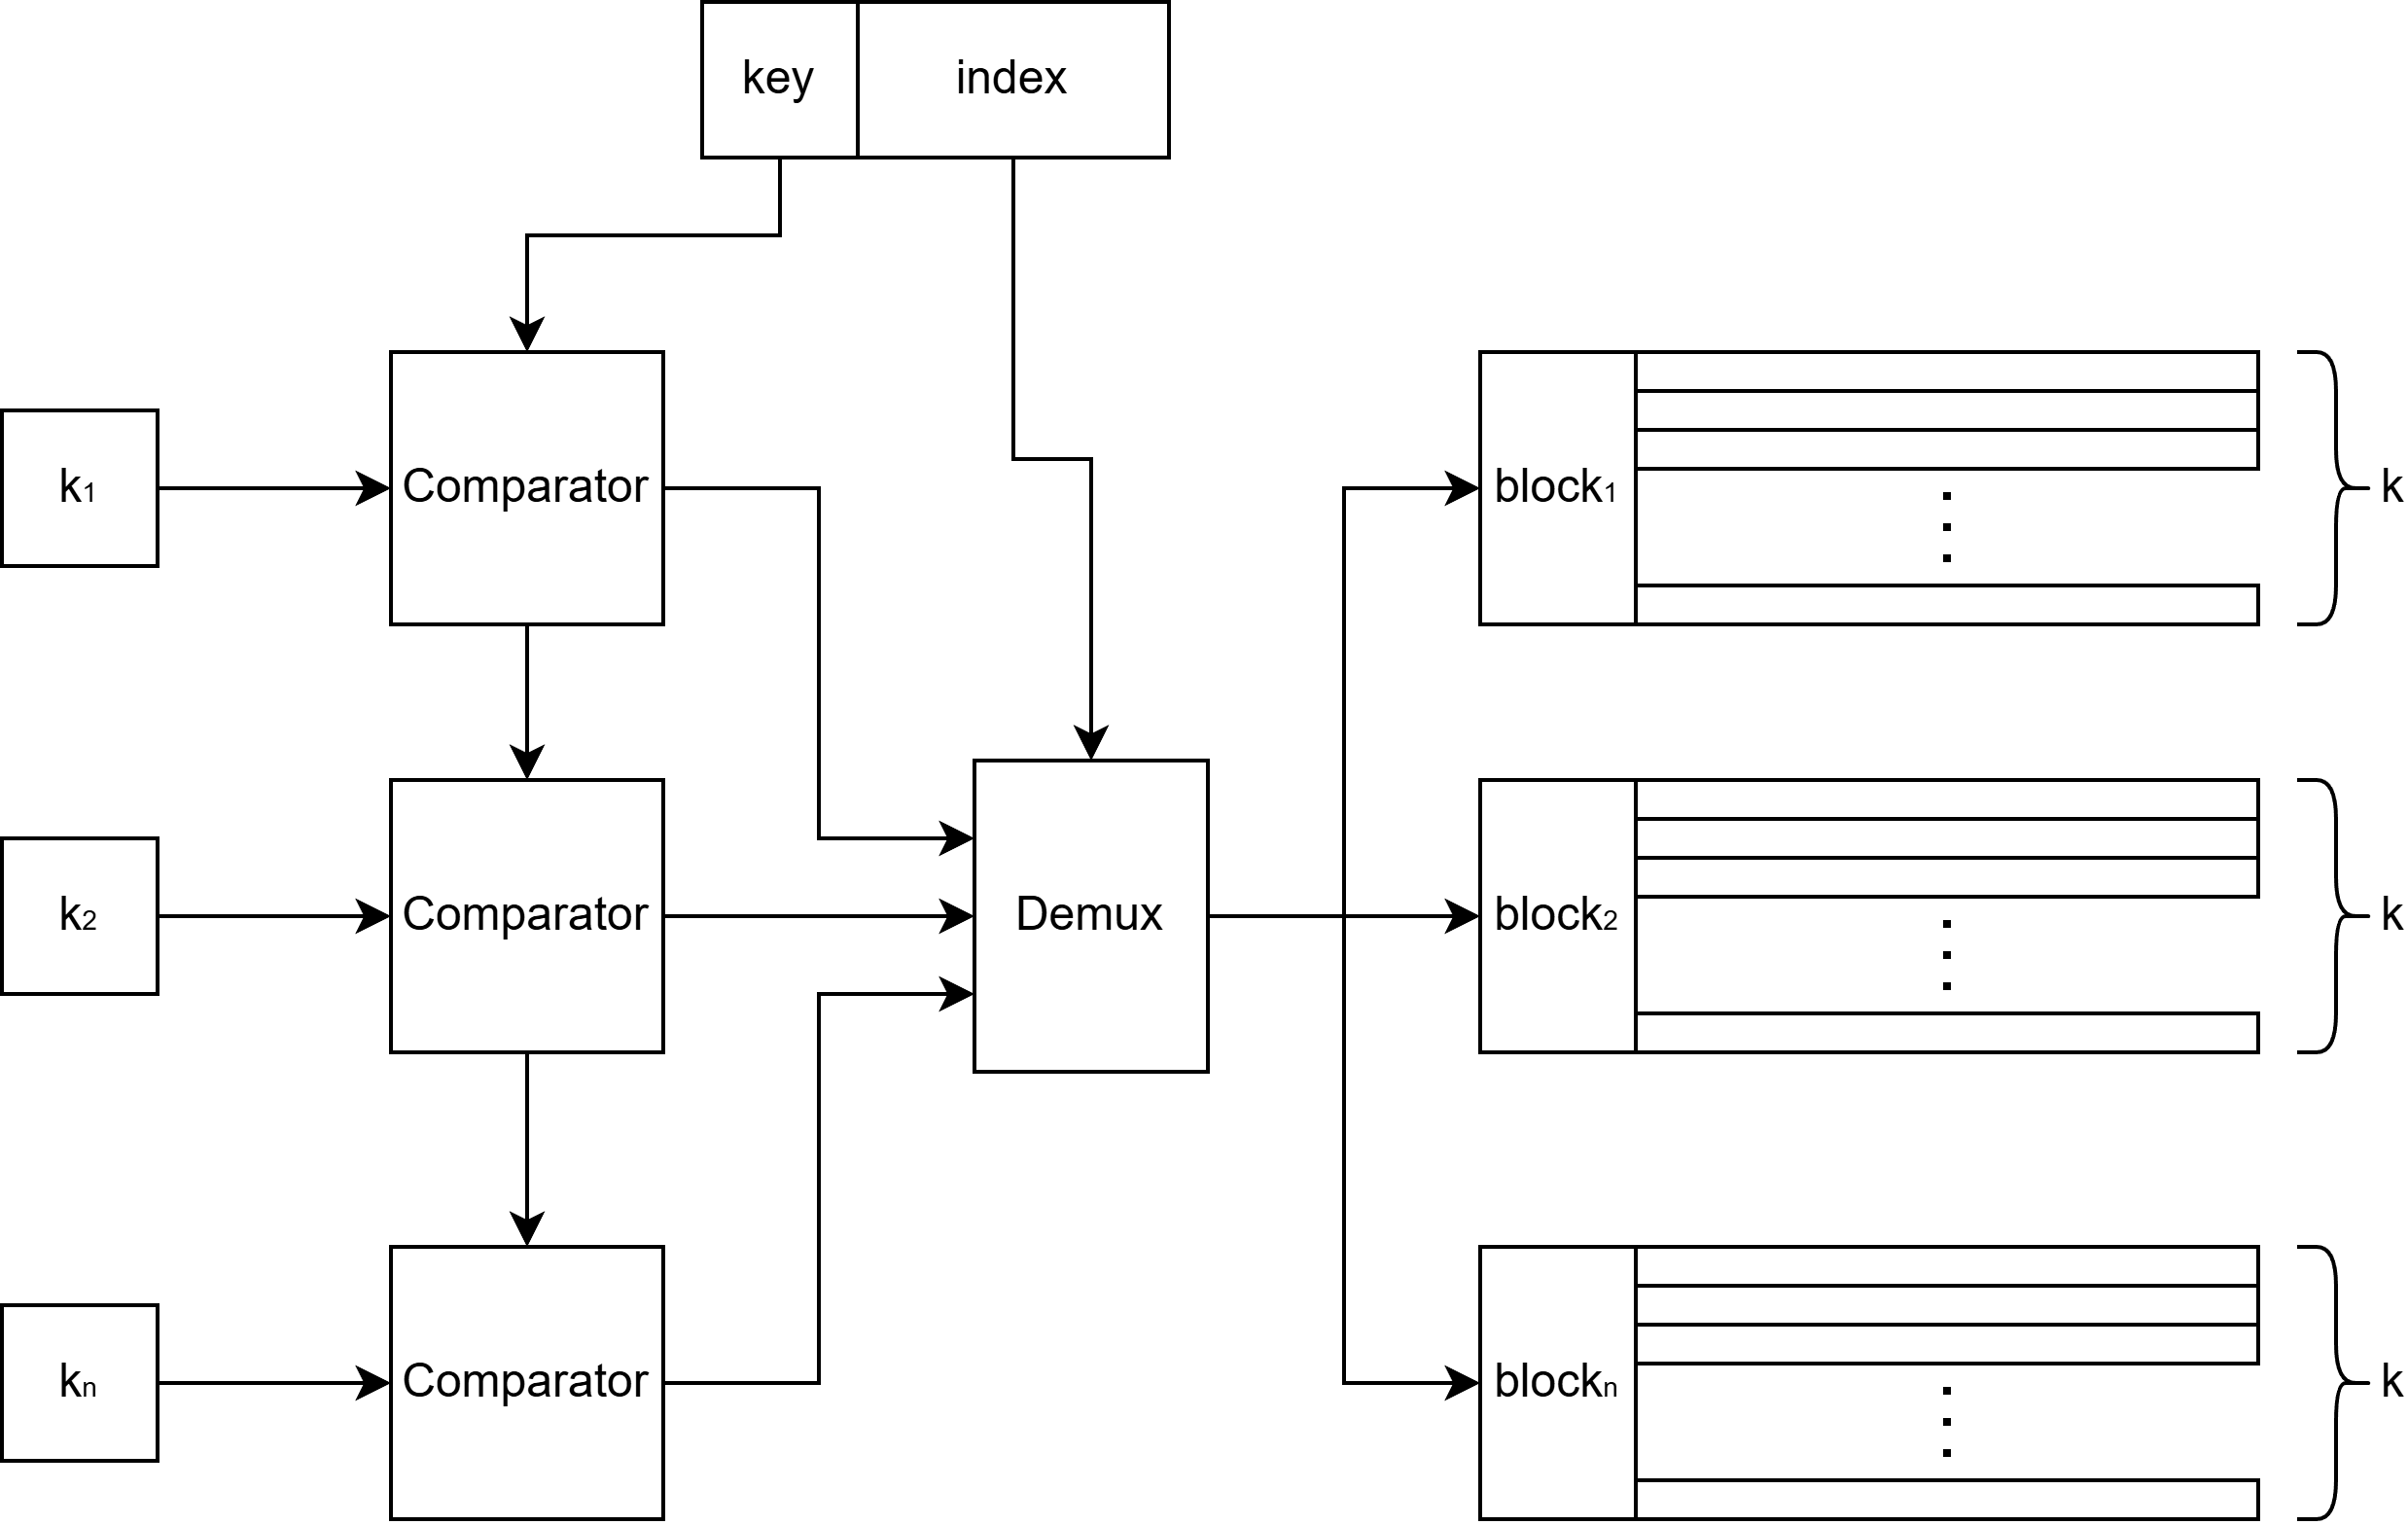
\includegraphics[width=0.7\linewidth]{img/full-assoc.png}
    \caption{Architettura di una memoria cache Full Associative.}
    \label{fig:full-ass}
\end{figure}

Cerchiamo di capire il motivo per cui una tale suddivisione degli indirizzi si rende necessaria. Come anticipato, le memorie cache sono caratterizzate da dimensioni molto ridotte, per cui se l'intero indirizzo venisse utilizzato per indicizzare un dato, si avrebbe uno spreco eccessivo (inefficienza). Ad esempio, se utilizzassimo indirizzi a 32 bit per indicizzare dati su 32 bit, il 50 dello spazio verrebbe sprecato per l'indirizzo.

\subsection{Politiche di Sostituzione}
Focalizziamo ora la nostra attenzione su cosa accade in caso di cache miss. In tale evenienza, la memoria cache deve interagire con la RAM per recuperare il dato mancante e sostituire uno dei suoi blocchi con uno contenente il dato appena prelevato. Questo processo può essere molto problematico nel caso in cui il programma esegue molti salti, a causa della continua sostituzione dei blocchi, ed è per questo motivo che un programma andrebbe scritto tenendo sempre presente il principio di località. Per quanto detto, la cache si comporta come un vero e proprio processore, in quanto interagisce con la RAM in caso di miss, ma come avviene la scelta della \textbf{politica di sostituzione}? Ovvero, come viene scelto il blocco da sostituire? Una prima semplice scelta potrebbe essere selezionare casualmente il blocco, una scelta leggermente più intelligente prevede di aggiungere un meccanismo che tenga conto di quanto ciascun blocco viene richiesto. Per poter implementare la seconda modalità, ciascun blocco memorizza, oltre ai dati, un bit di flag per la validità e due bit di conteggio. Ogni volta che un blocco viene utilizzato, i bit di conteggio sono azzerati, mentre ad ogni accesso in cache per cui il blocco non è richiesto, il valore di conteggio si incrementa. Quando è necessario sostituire un blocco, si sceglie quello con valore di conteggio più elevato (quello più vecchio) e in caso di pareggi si può utilizzare la scelta randomica. Il bit di validità è fondamentale all'avvio del sistema, in cui i dati presenti nei blocchi sono spazzatura e saranno quindi necessari diversi cache miss per poter portare la cache in uno stato "corretto". Ulteriori politiche di sostituzione prevedono l'impiego di algoritmi di tipo Round Robin e FIFO.

\subsection{Gestione dell'allineamento}
I dati presenti in cache potrebbero non corrispondere, e quindi non essere allineati, con quelli presenti nella RAM. Notiamo come il problema non si verifichi quando sono effettuate letture, ma esclusivamente in presenza di operazioni di scrittura. Sono evidentemente necessarie delle tecniche di \textbf{gestione dell'allineamento}. Le due principali soluzioni adottate sono:
\begin{itemize}
    \item \textbf{Write Through}: Ogni volta che viene scritta una parola in cache, in parallelo si effettua anche la scrittura in RAM. Dunque, le memorie risulteranno sempre allineate.
    \item \textbf{Write Back}: L'allineamento con la versione della parola in RAM avviene soltanto se il blocco in cui questa è contenuta è stato modificato, e la scrittura avviene prima che il blocco venga sostituito. Per realizzare questa tecnica è necessario aggiungere un ulteriore bit di modifica, oltre a quelli necessari per la politica di sostituzione. Quando il bit è alto, oltre a sostituire il blocco è necessario anche scrivere in RAM la versione aggiornata, per cui le due memoria non sono sempre allineate.
\end{itemize}

Notiamo come l'aggiunta di un DMA potrebbe complicare il progetto del sistema a seconda della soluzione di allineamento adottata. Nel caso del WT, il DMA può attivarsi immediatamente in quanto i dati sono sempre allineati, ma il bus viene utilizzato moltissimo, poiché ogni scrittura in cache comporta una corrispondente scrittura in RAM. Nel caso di WB, invece, prima di avviare il DMA è necessario forzare l'allineamento dei dati. 
\\
\\
Come possiamo immaginare, più la cache è vicina al processore e minore saranno i tempi di propagazione dei chip (maggiore velocità). Tuttavia, questo ha una limitazione in termini di dimensione della cache, in quanto più vicina questa sarà alla CPU, minore dovrà essere lo spazio occupato. Per questo motivo, nei sistemi moderni si utilizzano cache di diversi livelli e che lavorano nella maggior parte dei casi in Write Back. Inoltre, è molto probabile che le cache a bordo (vicine al processore) si trovino su processori di tipo RISC.

\subsection{Set Associative}
Una delle scelte più difficili riguardo l'architettura delle memorie cache riguarda la dimensione dei blocchi. Ad esempio, se il programma in esecuzione è molto locale, allora avere pochi blocchi molto grandi è sicuramente conveniente, mentre se il programma è poco locale la cosa migliore è avere molti blocchi piccoli. Osserviamo anche che maggiore è la dimensione dei blocchi, maggiore è la quantità di dati da trasferire in caso di cache miss, dunque idealmente vorremmo tanti blocchi piccoli per velocizzare gli spostamenti. Tuttavia, avere un numero elevato di blocchi porta fondamentalmente a due complicazioni:
\begin{enumerate}
    \item Il numero di comparatori necessari per la verifica della chiave cresce.
    \item Avere un elevato numero di chiavi porta al problema di inefficienza introdotto prima (spreco troppo spazio per memorizzare le chiavi).
\end{enumerate}

\MakeUppercase{è} fondamentale trovare dunque un giusto compromesso, cosa possibile complicando leggermente l'architettura delle memorie cache vista in precedenza e introducendone una di tipo \textbf{Set Associative}. Tale architettura può essere immaginata come una via di mezzo tra cache diretta (semplice ma rigida) e completamente associativa (flessibile ma costosa). Questa volta, la cache viene suddivisa in più set, ognuno dei quali contiene molteplici blocchi. Un dato può essere memorizzato in qualsiasi blocco del set, ma la ricerca avviene soltanto nel set giusto e non in tutta la memoria come avviene in quelle completamente associative. Per poter realizzare questo funzionamento, l'indirizzo fornito dal processore deve ora essere scomposto in tre parti: la prima identifica la chiave del blocco, la seconda il set in cui cercare e la terza l'offset rispetto al blocco [\ref{fig:indirizzo-setass}]. 

\begin{figure}[!h]
    \centering
    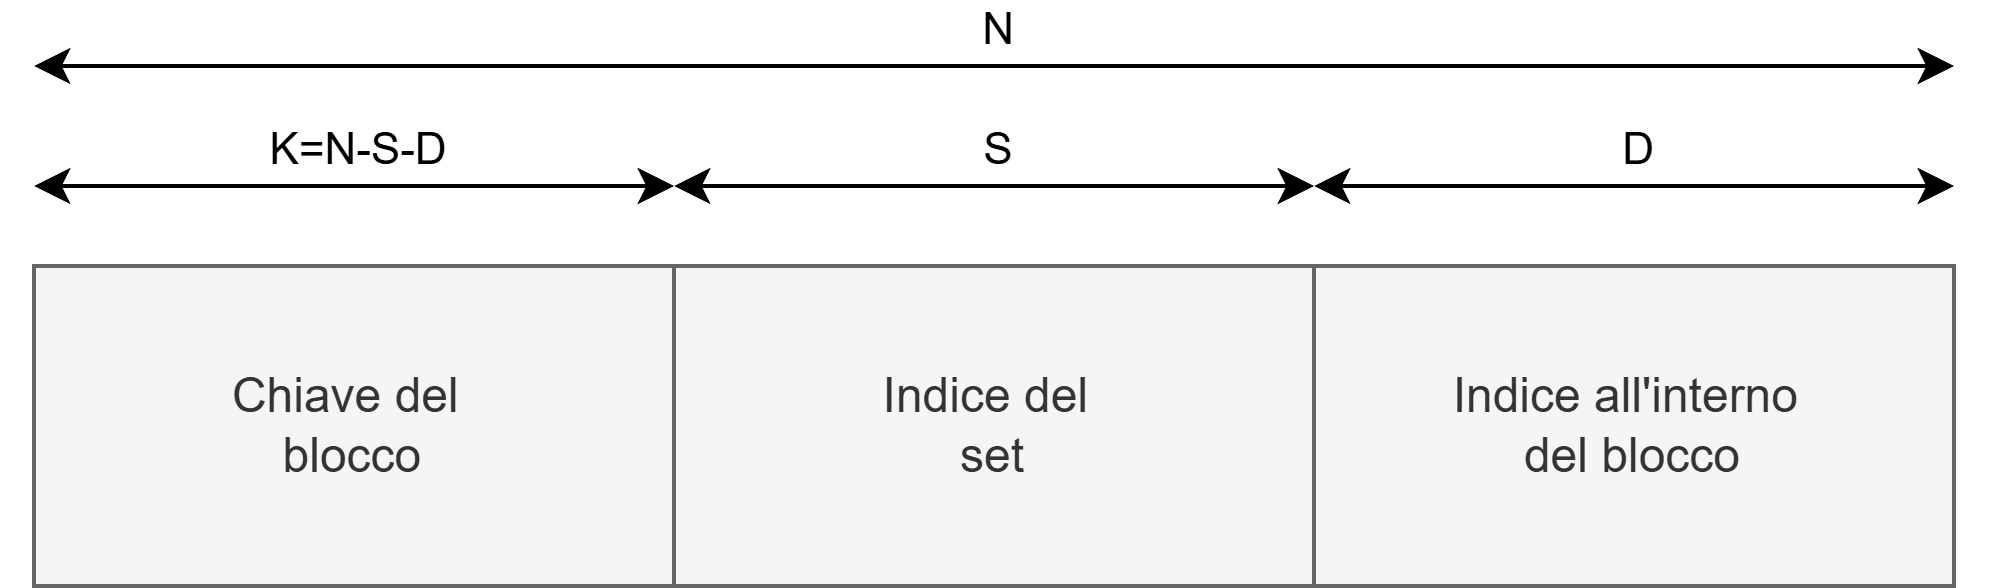
\includegraphics[width=0.6\linewidth]{img/indirizzo-setass.png}
    \caption{Struttura dell'indirizzo utilizzato per memorie cache set associative.}
    \label{fig:indirizzo-setass}
\end{figure}

La ricerca di un dato in cache avviene in due fasi: 
\begin{enumerate}
    \item \textbf{Selezione del set}: Utilizzando i bit dell'indirizzo destinati all'indice del set, un decoder seleziona l’insieme (set) corretto di blocchi della cache. Solo i blocchi di questo set saranno coinvolti nella ricerca. 
    \item \textbf{Confronto delle chiavi}: All'interno del set selezionato, i tag (le chiavi) di tutti i blocchi vengono confrontati in parallelo con il tag calcolato dall’indirizzo. Questo confronto determina se il blocco cercato è presente (cache hit) o meno (cache miss).
\end{enumerate}
Per ragioni di efficienza, questa architettura prevede che tutti i confronti sulle chiavi del set vengano effettuati in parallelo e che, mediante i D bit, i dati di tutti i blocchi contenuti nel set individuato vengano comunque selezionati, ma al processore sarà trasmesso soltanto il dato appartenente al blocco per il quale si è verificata la corrispondenza tra le chiavi. In questo modo, la selezione del dato nel blocco e la verifica della corrispondenza tra chiavi può essere fatta in parallelo. Ovviamente, nel caso in cui non si riscontri alcuna corrispondenza tra le chiavi, si avrà un miss e il dato dovrà essere prelevato dalla RAM (o dalla memoria superiore nel sistema gerarchico).
\\
\\
All'inizio del capitolo è stato affermato che un'architettura Set Associative consente un risparmio in termini di numero di comparatori e di lunghezza delle chiavi, rispetto a un'organizzazione completamente associativa. Vediamo ora in che modo ciò avviene. Consideriamo, a parità di lunghezza dell'indirizzo N, una cache completamente associativa e una set-associativa. 
\begin{enumerate}
    \item Nel caso completamente associativo, non esistendo un campo indice per selezionare un set, la lunghezza del campo chiave sarà pari a K=N-D, dove D rappresenta il numero di bit usati per l'offset all'interno del blocco.
    \item Nel caso set-associativo, parte dell'indirizzo viene utilizzata per selezionare il set: supponendo di avere \(2^s\) set, la lunghezza del campo chiave si riduce a K=N-S-D.
\end{enumerate}
Ne consegue che l'organizzazione Set Associative richiede meno bit per ogni tag, e, poiché la ricerca viene effettuata solo sui blocchi appartenenti al set selezionato, sono necessari meno comparatori rispetto all'organizzazione Full Associative, dove il confronto deve avvenire con tutti i blocchi della cache.

\subsection{Dimensionamento}
Dimensionare un sistema significa determinare le sue caratteristiche fisiche sulla base dell'architettura studiata. Consideriamo, in particolare, il \textbf{dimensionamento di una memoria cache}. In questo contesto, è necessario definire tre parametri fondamentali: il numero di blocchi (\(k\)), il numero di settori (\(s\)) e la lunghezza di ciascun blocco (\(L\)). La dimensione complessiva della cache si ottiene come prodotto di questi fattori, \(dim=ksL\). È utile osservare che il dimensionamento della memoria virtuale, tema di maggiore interesse nei nostri studi, può essere interpretato come un caso particolare del dimensionamento della cache, data la somiglianza strutturale tra le due tipologie di memoria.
\\
\\
L’obiettivo del dimensionamento è minimizzare il numero di cache miss. Tuttavia, non esiste una configurazione ottimale valida in assoluto, poiché le prestazioni della cache dipendono fortemente da fattori quali la località del programma e i dati di input utilizzati. Per affrontare questa variabilità, i tool di dimensionamento automatico (come SPIM) testano il sistema con diverse tipologie di applicazioni, per valutare il comportamento della cache in una vasta gamma di situazioni. In generale, il rapporto tra la dimensione della cache e il numero di cache miss può essere rappresentato graficamente, mostrando come l’aumento della dimensione influenzi (non sempre linearmente) il tasso di miss [\ref{fig:graph_cache}].

\begin{figure}[!h]
\begin{center}
\begin{tikzpicture}
  \begin{axis}[
    axis lines=middle,
    xlabel={dim},
    ylabel={cache miss},
    xmin=0, xmax=10,
    ymin=0, ymax=1.2,
    samples=200,
    domain=0.1:10,
    thick,
    every axis y label/.style={at={(axis description cs:0, 1.02), anchor=south}, anchor=south},
    every axis x label/.style={at={(current axis.right of origin)}, anchor=west}
  ]
    \addplot[black] {1/x};
  \end{axis}
\end{tikzpicture}
\end{center}
\caption{Grafico di dimensionamento della memoria cache.}
\label{fig:graph_cache}
\end{figure}

Per dimensionare correttamente la cache, è importante individuare un punto nel grafico che consenta di mantenere costante il numero di cache miss, evitando però una dimensione eccessiva della memoria. In pratica, i tool di dimensionamento ripetono questa analisi per ciascuna delle applicazioni in ingresso, valutando una configurazione che rappresenti una media ottimizzata. Naturalmente, il dimensionamento non può prescindere dai vincoli di realizzabilità fisica, trasformando il problema in un problema di ottimo vincolato.
\\
\\
Il problema, come definito, si presenta con una sola equazione e tre incognite, il che implica un numero infinito di soluzioni possibili. Tuttavia, molti di questi casi possono essere esclusi in base a vincoli fisici o pratici. Possiamo ulteriormente ridurre il numero di combinazioni imponendo vincoli sui singoli parametri. Ad esempio:
\begin{enumerate}
    \item Il numero di blocchi \(k\) può assumere valori discreti e non troppo grandi, come 4, 8 o 16, a causa dei problemi di gestione di un numero eccessivo di blocchi.
    \item La dimensione dei blocchi \(L\) non può essere arbitrariamente grande, spesso viene scelta proporzionalmente al numero di blocchi, ad esempio \(L=pk\).
    \item Una volta fissati \(k\) e \(L\), il numero di set \(s\) risulta vincolato dagli altri due parametri.
\end{enumerate}

Nonostante questi vincoli, il numero di combinazioni possibili rimane elevato, rendendo impraticabile una ricerca esaustiva. Per questo motivo, si ricorre spesso a euristiche, basate su osservazioni statistiche del comportamento tipico della cache: si cerca di stimare la probabilità di cache miss dato un certo applicativo e una configurazione specifica della cache. Infine, notiamo che è possibile ridurre ulteriormente il numero di simulazioni necessarie. Se, per esempio, è già disponibile una simulazione per \(k=4\), possiamo inferire anche quella per \( k=2\). In effetti, ciò presuppone un'ipotesi forte: che il comportamento della cache non cambi in modo significativo al variare della sua dimensione. Questa semplificazione è spesso accettata per rendere il problema trattabile.